\documentclass[tikz, border=15pt]{standalone}
\usepackage{amsmath}
\usetikzlibrary{positioning, arrows.meta, shapes.geometric, calc, backgrounds, fit}

\begin{document}
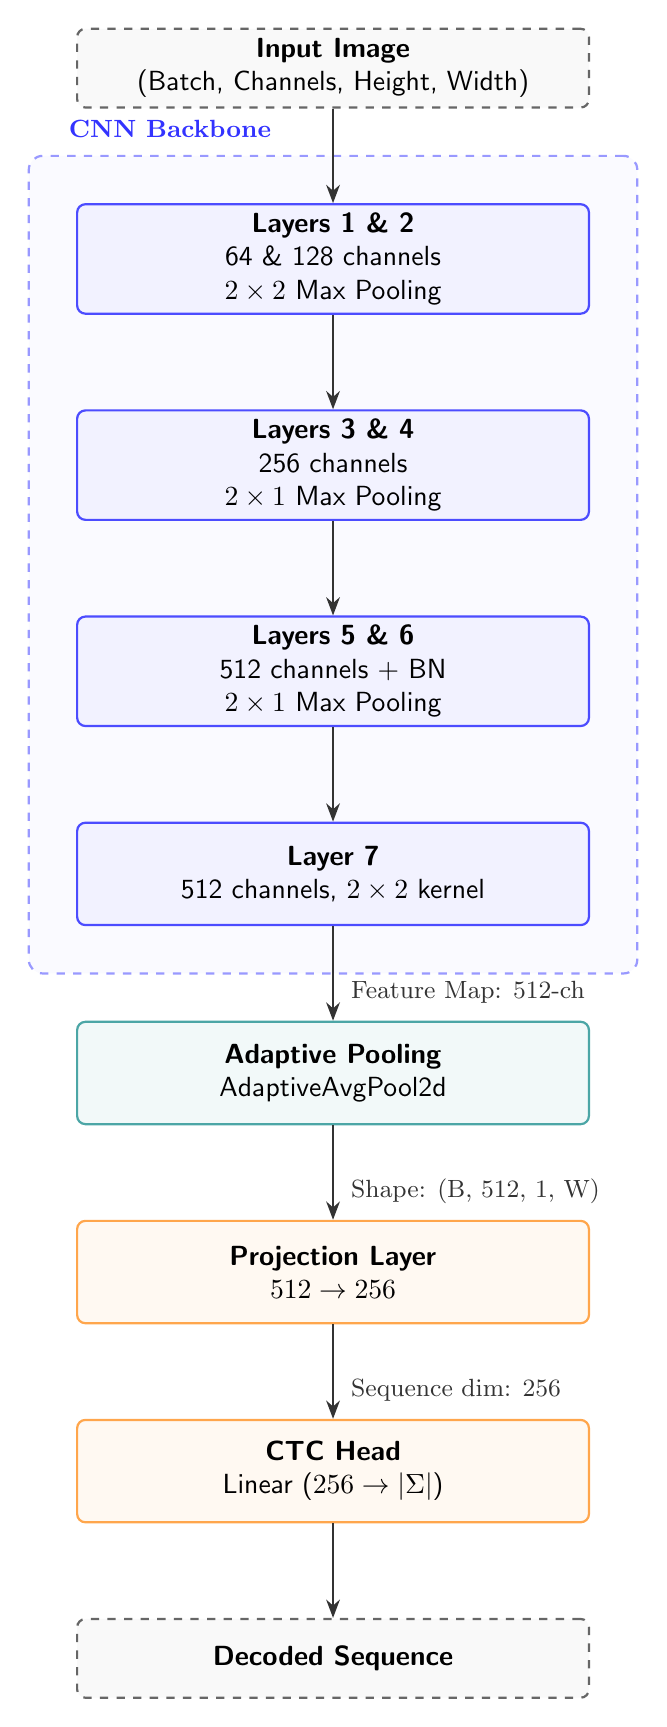
\begin{tikzpicture}[
    font=\sffamily,
    >=Stealth,
    % INCREASED node distance from 0.9 to 1.4 for longer arrows
    node distance=1.2cm and 0.4cm,
    block/.style={
        draw=black!70, thick,
        rectangle, rounded corners=3pt,
        minimum width=6.5cm, minimum height=1.3cm,
        align=center, fill=white
    },
    cnn/.style={block, fill=blue!5, draw=blue!70},
    pool/.style={block, fill=teal!5, draw=teal!70},
    fc/.style={block, fill=orange!5, draw=orange!70},
    io/.style={
        draw=black!60, thick, dashed,
        rectangle, rounded corners=3pt,
        minimum width=6.5cm, minimum height=1cm,
        align=center, fill=gray!5
    },
    arrow/.style={->, thick, draw=black!80},
    % Added 'midway' and 'xshift' to the label style for better clearance
    label node/.style={align=left, font=\small\color{black!80}, anchor=west, xshift=0.1cm}
]

% Nodes
\node[io] (input) {\textbf{Input Image} \\ (Batch, Channels, Height, Width)};
\node[cnn, below=of input] (l12) {\textbf{Layers 1 \& 2} \\ 64 \& 128 channels \\ $2\times2$ Max Pooling};
\node[cnn, below=of l12] (l34) {\textbf{Layers 3 \& 4} \\ 256 channels \\ $2\times1$ Max Pooling};
\node[cnn, below=of l34] (l56) {\textbf{Layers 5 \& 6} \\ 512 channels + BN \\ $2\times1$ Max Pooling};
\node[cnn, below=of l56] (l7) {\textbf{Layer 7} \\ 512 channels, $2\times2$ kernel};
\node[pool, below=of l7] (adp) {\textbf{Adaptive Pooling} \\ AdaptiveAvgPool2d};
\node[fc, below=of adp] (proj) {\textbf{Projection Layer} \\ $512 \rightarrow 256$};
\node[fc, below=of proj] (ctc) {\textbf{CTC Head} \\ Linear ($256 \rightarrow |\Sigma|$)};
\node[io, below=of ctc] (output) {\textbf{Decoded Sequence}};

% Arrows with manual spacing adjustments
\draw[arrow] (input) -- (l12);
\draw[arrow] (l12) -- (l34);
\draw[arrow] (l34) -- (l56);
\draw[arrow] (l56) -- (l7);

% Using 'midway' ensures the text is centered on the now-longer arrow
\draw[arrow] (l7) -- node[pos=0.7, label node] {Feature Map: 512-ch} (adp);
\draw[arrow] (adp) -- node[pos=0.7, label node] {Shape: (B, 512, 1, W)} (proj);
\draw[arrow] (proj) -- node[pos=0.7, label node] {Sequence dim: 256} (ctc);
\draw[arrow] (ctc) -- (output);

% Background Box Adjustment
\begin{scope}[on background layer]
    \node[fit=(l12)(l7), draw=blue!40, fill=blue!2, thick, dashed, rounded corners=5pt, inner sep=0.6cm] (cnn_box) {};
    % Added yshift to move the label AWAY from the top of the box
    \node[anchor=south west, font=\small\bfseries\color{blue!80}, shift={(0.4, 0.1)}] at (cnn_box.north west) {CNN Backbone};
\end{scope}

\end{tikzpicture}
\end{document}